\section{3d Welt}\label{sec:3d-world}
\setauthor{Florian Beckerle}
Jedes Spiel besitzt eine Spielwelt.
Dabei ist es egal ob es sich um eine 3D oder 2D Applikation handelt.
Unter den Begriff Spielwelt fällt die Umgebung in welcher, sich der Spieler befindet.
Es gibt hierbei so gut wie keine Einschränkungen in Bezug auf Kreativität, egal ob die digitale Welt nun ein riesiger Ring, der im Weltall schwebt,
oder eine verlassene Großstadt in einer postapokalyptischen Welt ist, siehe Abb. ~\ref{fig:3d_environment_destiny2}.
~\cite{GamesRadar_HaloRing_2022}



%% this image and the next are not working. see issue #1

\begin{figure}
    \centering
    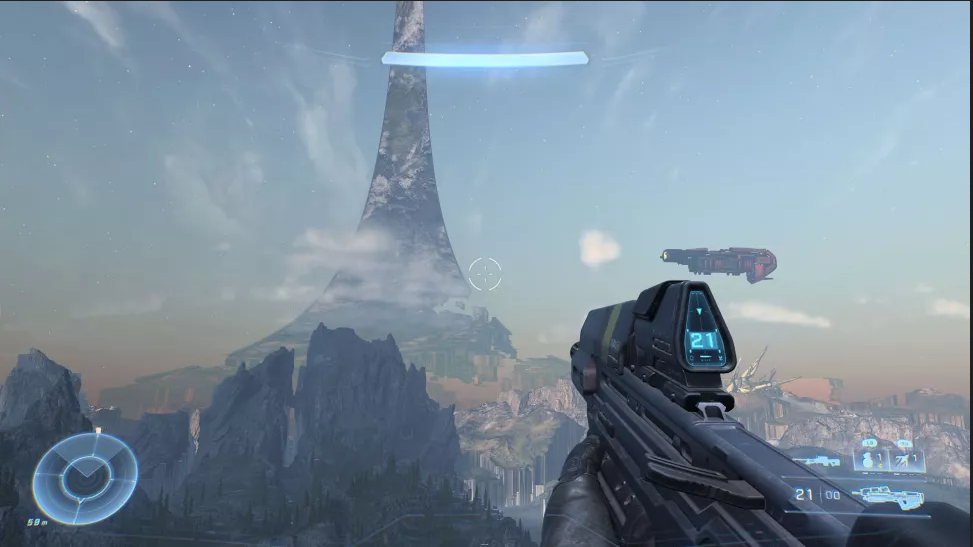
\includegraphics[scale=0.4]{pics/3d_welt_halo_ring}
    \caption{3D Welt - Halo}
    \label{fig:3d_environment_halo}
\end{figure}


%% Grafik für Destiny 2 Locations noch einbinden (Seite für Quelle lädt grade nicht Bungie.net)

\begin{figure}
    \centering
    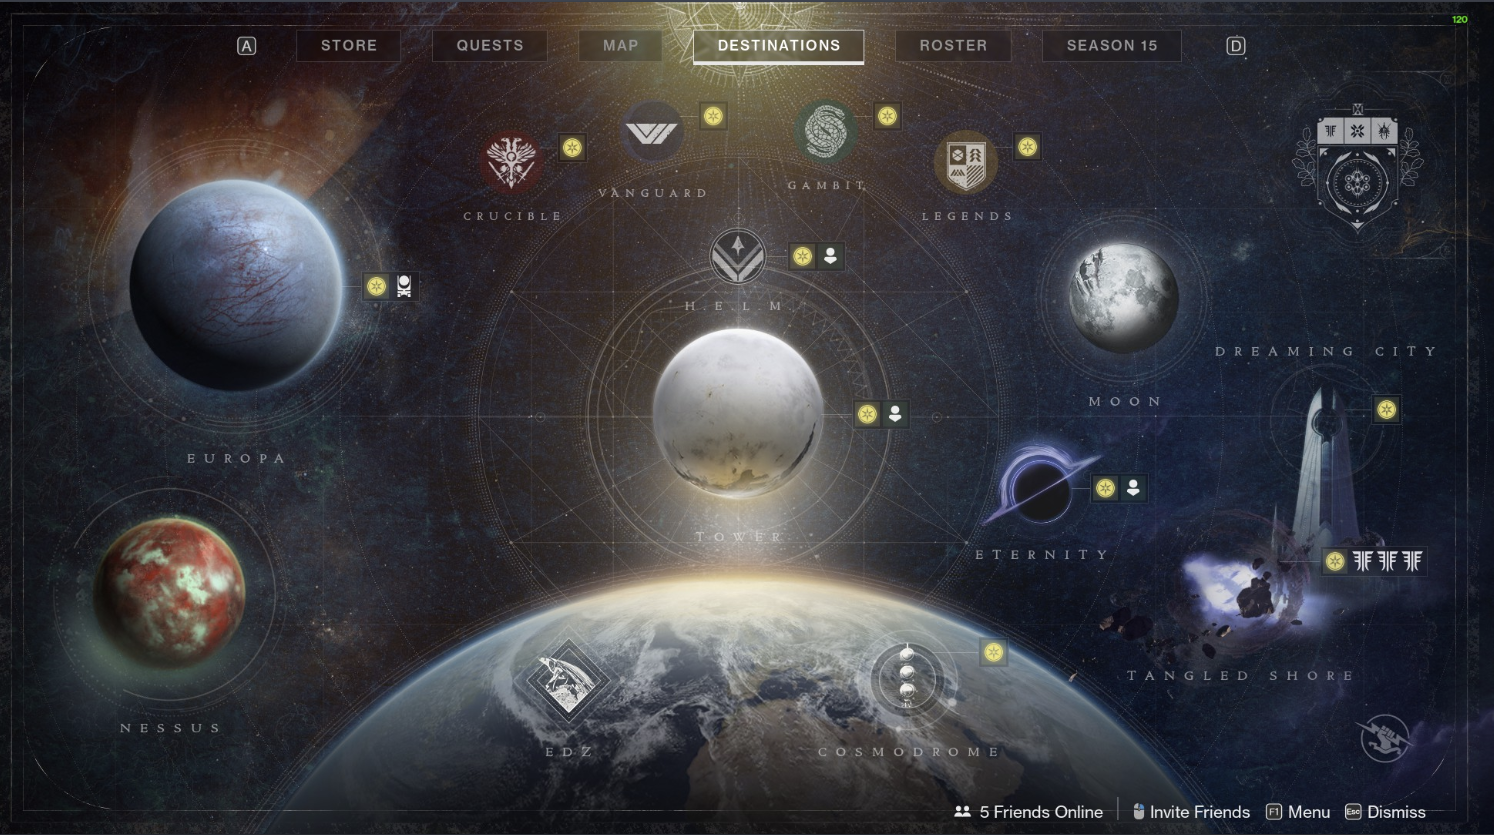
\includegraphics[scale=0.3]{pics/3d_welt_destiny_planets}
    \caption{3D Welt - Destiny 2}
    \label{fig:3d_environment_destiny2}
\end{figure}

Spielehersteller bauen die Spielwelten so auf, wie es am besten zu der Vision des Spieles passt.
Gleichzeitig wird darauf geachtet, dass sich die Umgebung nicht langweilig oder leer anfühlt.
Hierfür wird Environmental Storytelling verwendet.
Darunter versteht man das Platzieren von Gegenständen und Objekten,
welche dem Spieler eine kleine Geschichte erzählen.
Das passiert jedoch nicht über Sprache sondern einfach nur über die Platzierung und das Aussehen.
Ein Beispiel hierfür w\"are das Bild von Cayde-6 (ein Charakter aus Destiny 2), welches in einem Restaurant platziert wurde.
Cayde ist einer der drei Anführer der Vanguard, welche eine Ansammlung an Guardians (Spielern und NPC) ist und gegen das Böse kämpft.
In Forsaken starb Cayde jedoch und viele trauerten um ihn, als Gedenken wurde dieses Bild aufgehängt.
~\cite{GameDeveloper_2022}

\begin {figure}
    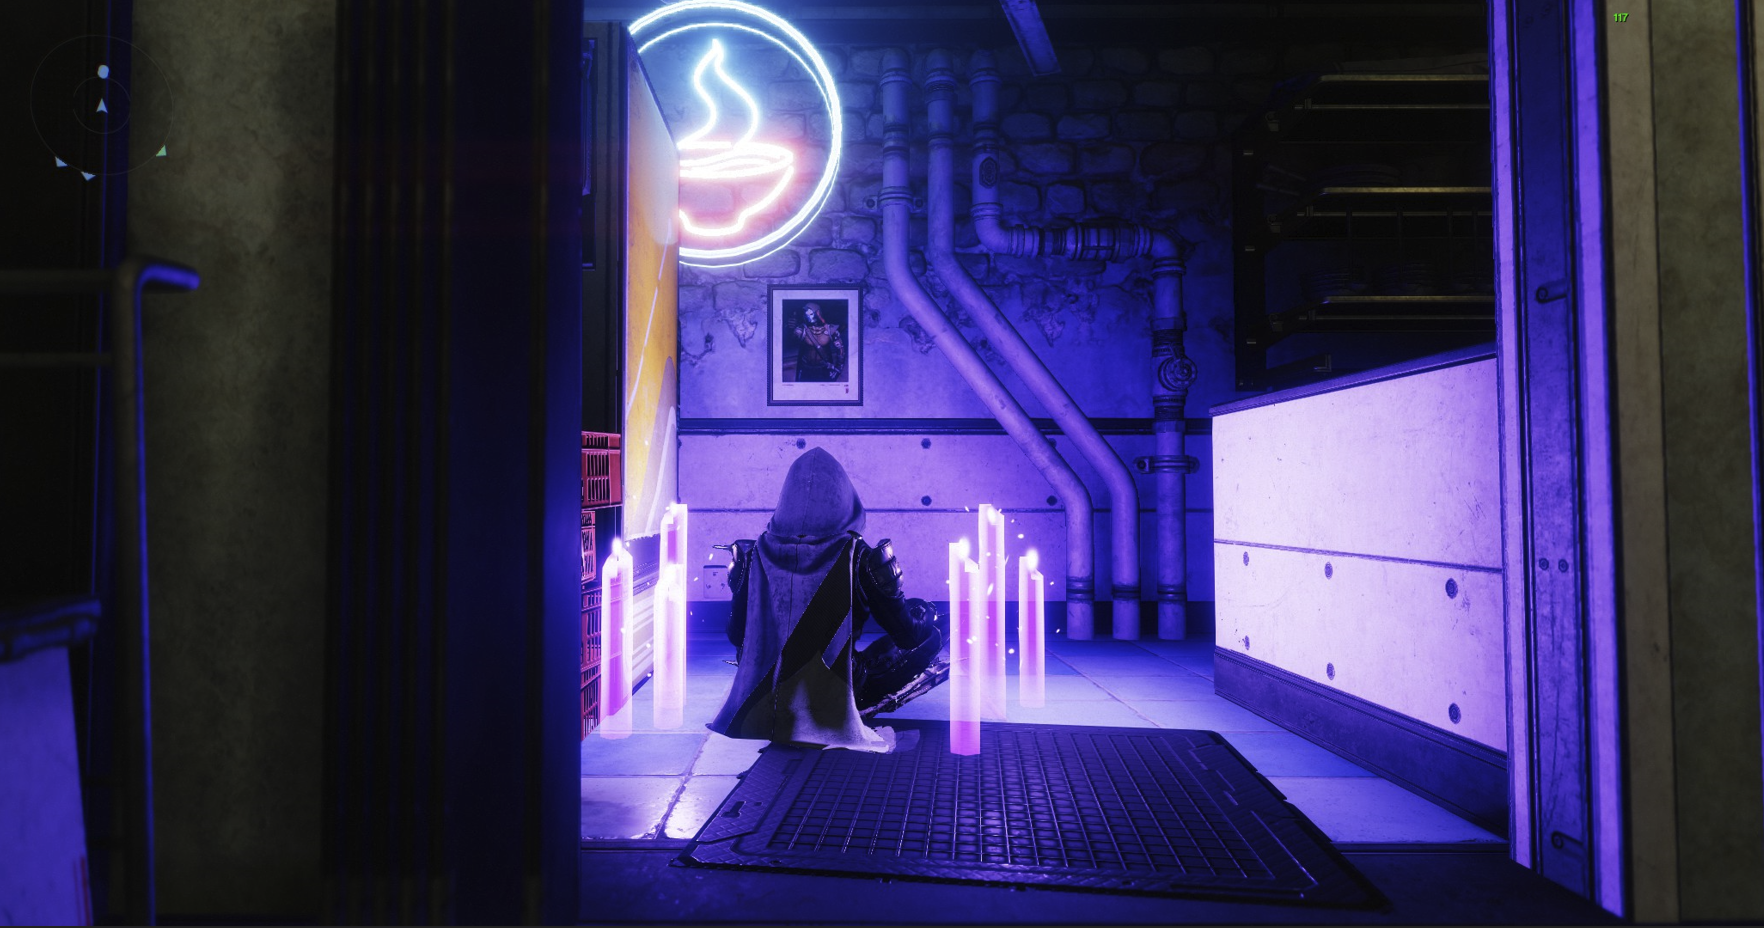
\includegraphics[scale=0.3]{pics/3d_welt_destiny2-environmental-storytelling}
    \caption{Environmental Storytelling '-' Destiny 2 Cayde}
    \label{fig:3d_environmental_storytelling_destiny2}
\end {figure}


\subsection{City Grid System}\label{subsec:city-grid-system}
\setauthor{Florian Beckerle}
Um die Gestaltung der Welt in BeamVR zu erleichtern, wurde ein Grid System verwendet.
Dafür ist die Stadt in ein Raster aufgeteilt, an welchem sich alle Objekte der Welt auf allen 3 Achsen (x,y,z) orientieren.
Unity stellt, wie in Abb. ~\ref{fig:grid-system-unity} zu sehen, so ein Grid Snapping System zur Verf\"ugung.
Daher wurde f\"ur BeamVR am Anfang der Modellierungsphase eine bestimmte Grid-Size festgelegt,
an welche die Grundfl\"achen der Geb\"aude und die Straßen
angepasst wurden.

\begin {figure}
    \centering
    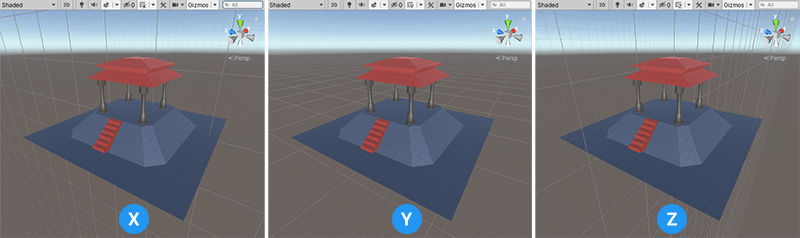
\includegraphics[scale=0.5]{pics/unity-grid-snapping}
    \caption{Unity '-' Grid Snapping System}
    \label{fig:grid-system-unity}
\end {figure}

Wenn man die Grid Size, also die Gr\"osse des Rasters \"andern m\"ochte, muss man zuerst im Editor das Grid and Snap Fenster öffnen.
Als n\"achstes findet man unter dem Bereich World Grid ein Attribut namens Size, wo man die X, Y und Z Achsen frei und unabh\"angig voneinander umskalieren kann, siehe Abb. ~\ref{fig:grid-size-unity}.
~\cite{Unity_GridSnapping_2022}

\begin {figure}
    \centering
    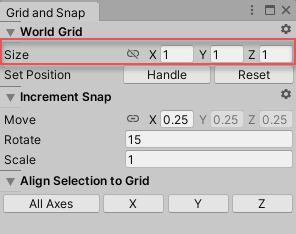
\includegraphics{pics/unity-grid-snapping-size}
    \caption{Unity - Grid Snapping Size}
    \label{fig:grid-size-unity}
\end {figure}



\subsection{Stadt}\label{subsec:city}
\setauthor{Florian Beckerle}
Jede Stadt hat viele verschiedene Strukturen wie zum Beispiel Sehensw\"urdigkeiten, Bauwerke und Einrichtungen wie Kinos, Theater oder Restaurants.
F\"ur BeamVR wurden daher insgesamt \"uber 34 Geb\"aude Modelle erstellt, um eine Vielfalt in der Umgebung zu erreichen, siehe Abb. ~\ref{fig:beamvr_building-variety}.

\begin {figure}
    \centering
    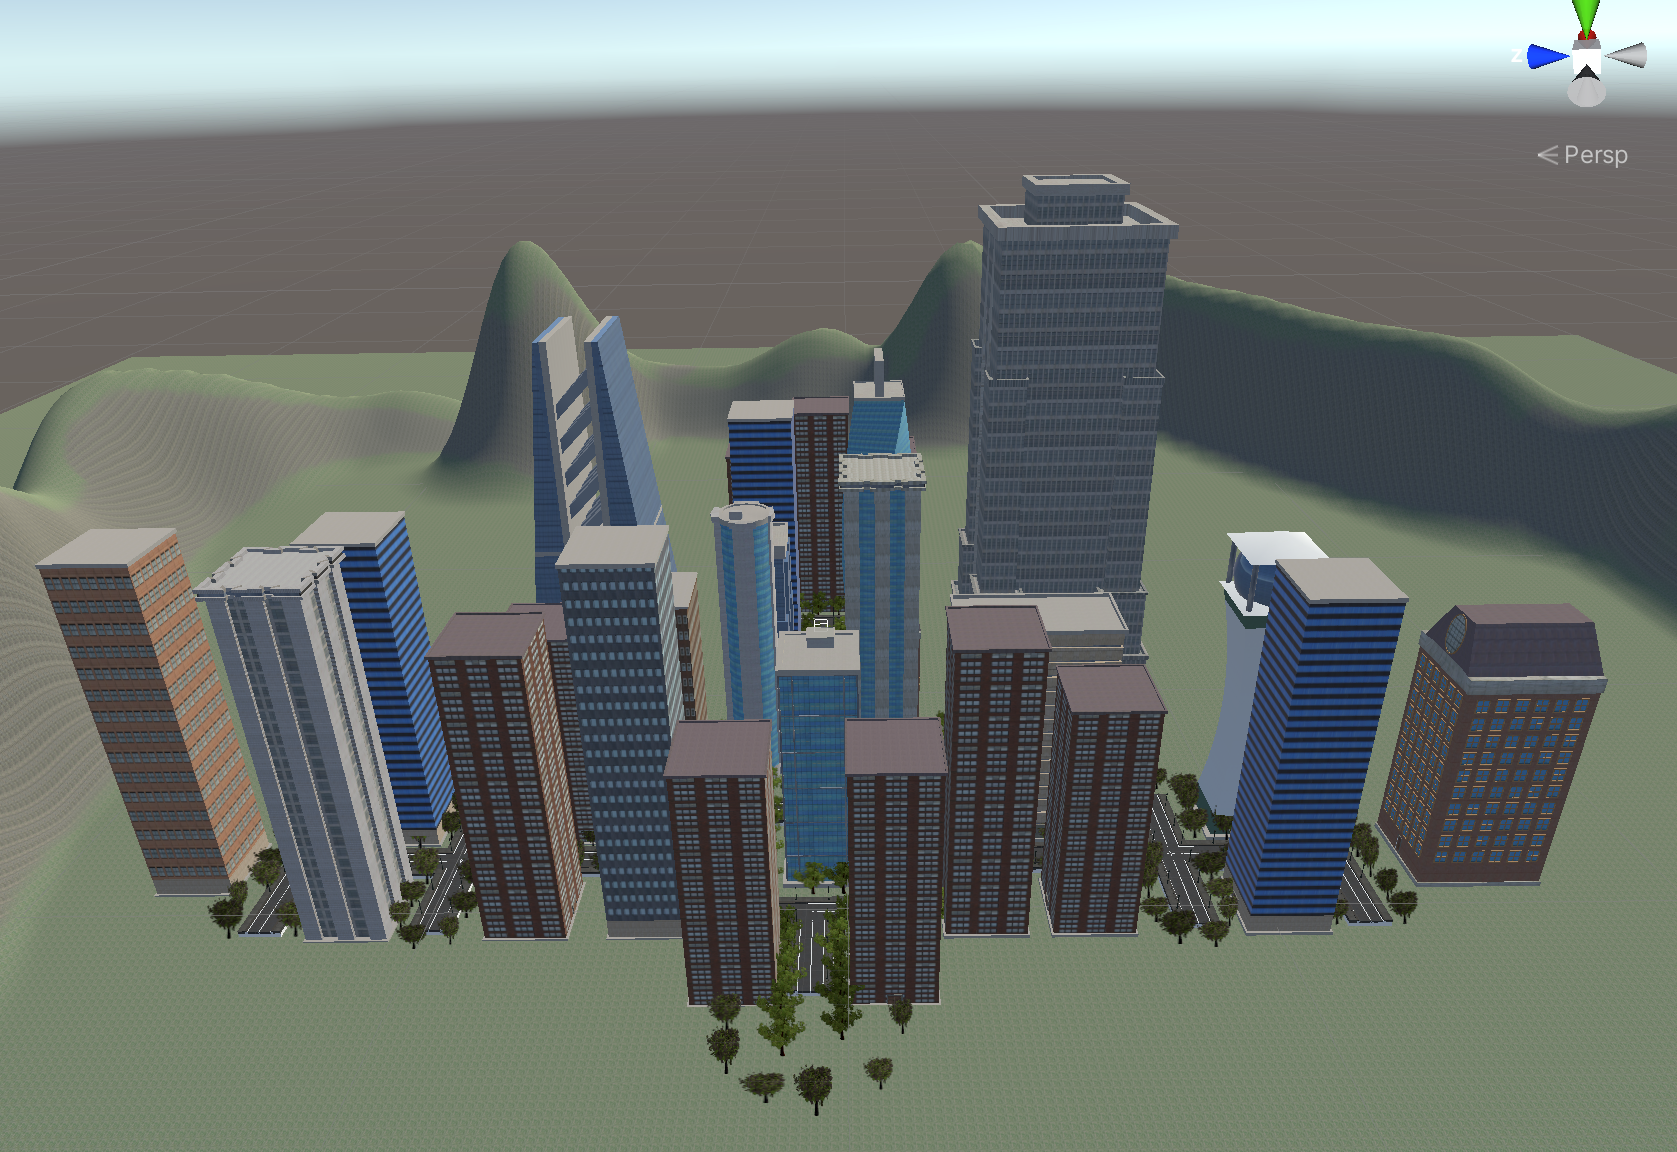
\includegraphics[scale=0.18]{pics/beamvr_building-variety}
    \caption{Beam VR - Building Overview}
    \label{fig:beamvr_building-variety}
\end {figure}

Die Stadt wurde so entworfen, dass nur die für den Spieler sichtbaren Objekte wirklich existieren, wie auf der Abb. ~\ref{fig:beamvr_building-variety} zu erkennen ist.
Bei richtiger Umsetzung scheint es für den Anwender dennoch so, als w\"are dieser in einer kompletten Spielwelt.
Um die Performance des Spieles zu verbessern, wurde dieser Trick in BeamVR angewandt, da unn\"otige Objekte nicht gerendert oder berechnet werden m\"ussen.
Bei gr\"oßeren Projekten spart das nicht nur Zeit sondern auch Ressourcen.
Bei BeamVR wurde diese Technik angewandt, um die Frames per Second zu erh\"ohen.

\subsection{Tag Stadt}\label{subsec:day-city}
\setauthor{Florian Beckerle}
Es wurden 17 der 34 unterschiedlichen Geb\"aude f\"ur diese Map modelliert, siehe Abb. ~\ref{fig:beamvr_building-variety}.
Der Fokus bei der Gestaltung der Bauwerke lag darauf, dass diese m\"oglichst realistisch aussehen und dennoch nicht zu rechenaufwendig in der Darstellung sind.
Daher wurden Texturen verwendet, um kleinere Details an den Fassaden darzustellen, statt diese zu modellieren.
Das gleiche Prinzip wurde bei der Apocalypse Map verwendet, siehe Abschnitt ~\ref{subsec:apocalypse-city}.
Die Texturen stellen Fassaden aus Stein und Glas dar.
Ein weiterer wichtiger Punkt bei der Planung der Stadt war es auch, dass der Spieler nicht aus der Stadt hinaus schauen kann und die Illusion aufrecht erhalten bleibt.
Daher wurden alle umliegenden Bauwerke mindestens 3 Meter h\"oher gemacht als das Geb\"aude, auf dem sich der Spieler befindet, siehe Abb. ~\ref{fig:beamvr_building-heights}.

\begin {figure}
    \centering
    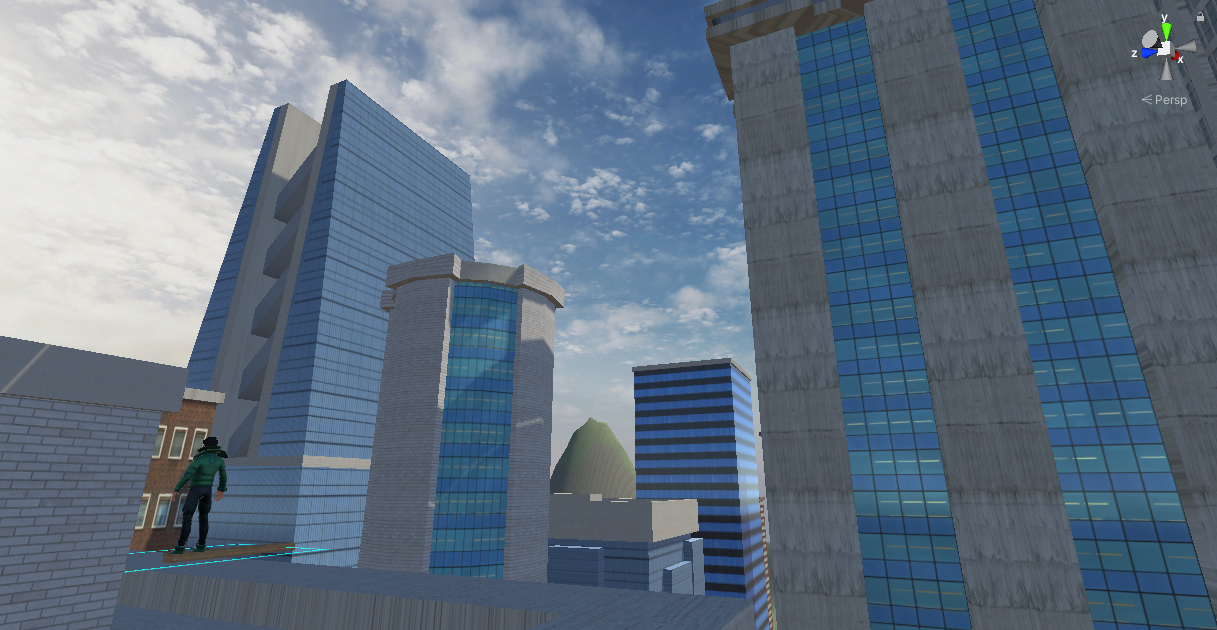
\includegraphics[scale=0.5]{pics/beamvr_city_day_heights}
    \caption{Beam VR - Building Heights}
    \label{fig:beamvr_building-heights}
\end {figure}

\subsection{Nacht Stadt}\label{subsec:night-city}
\setauthor{Florian Beckerle}
In der Nacht Version der Stadt wurde die Skybox angepasst.
Diese zeigt nun einen Sternenhimmel.
Es handelt sich hierbei um eine Sphere oder Box, welche sich um die Spielwelt befindet.
Sie wird dazu benutzt, um einen Himmel oder andere Umgebungen,
in Form von Texturen darstellen zu können, ohne dass diese als Modelle existieren.
Zus\"atzlich wurde die Belichtung der Scene auf ein bl\"auliches Licht eingestellt und die Laternen in den Straßen
haben noch eigene Lichtquellen, siehe Abb. ~\ref{fig:beamvr_night_map_lighting}.

\begin {figure}
    \centering
    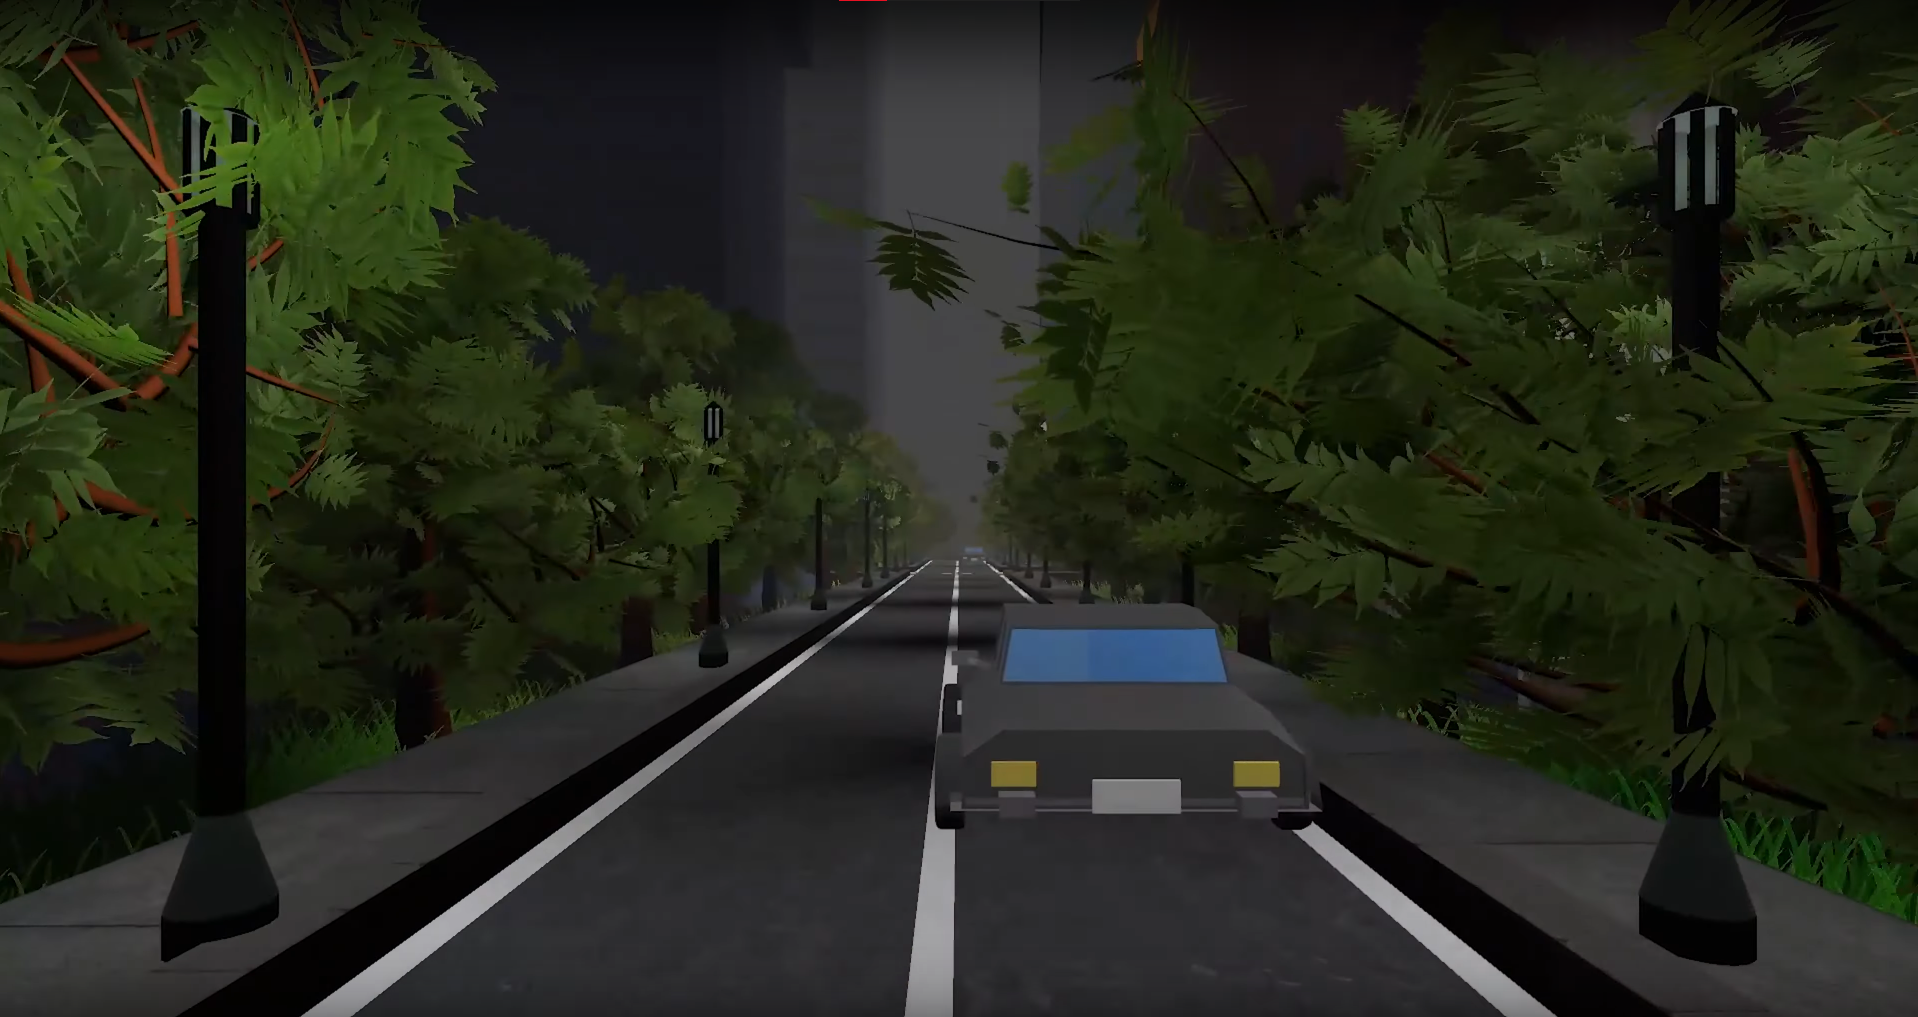
\includegraphics[scale=0.3]{pics/beamvr_night_overview}
    \caption{Beam VR - Night Map Lighting}
    \label{fig:beamvr_night_map_lighting}
\end {figure}

\subsection{Apocalypse Stadt}\label{subsec:apocalypse-city}
\setauthor{Florian Beckerle}
F\"ur diese Umgebung wurden alle Geb\"aude nocheinmal \"uberarbeitet.
Statt der intakten Glasfassaden werden nun barrikadierte Fenster und Ziegelsteine ohne Verputz f\"ur die Bauwerke verwendet, siehe Abb. ~\ref{fig:beamvr_damaged_texture}.
Durch diese \"Anderung sieht die Stadt verlassen und postapokalyptisch aus.
Um den Effekt noch zus\"atzlich zu verst\"arken, wurden die Bauwerke in eine Schieflage gebracht, sodass es aussieht, als w\"urden diese gleich zusammenbrechen.
Das Gel\"ande wurde mit neuen Sandstein Texturen und D\"unen in eine W\"uste umgewandelt.
Die Planzen und B\"aume wurden durch ausgetrocknete B\"usche ausgetauscht, damit die Welt ein trostloses Aussehen erhält, siehe Abb. ~\ref{fig:beamvr_apocalypse_map}.

\begin {figure}
    \centering
    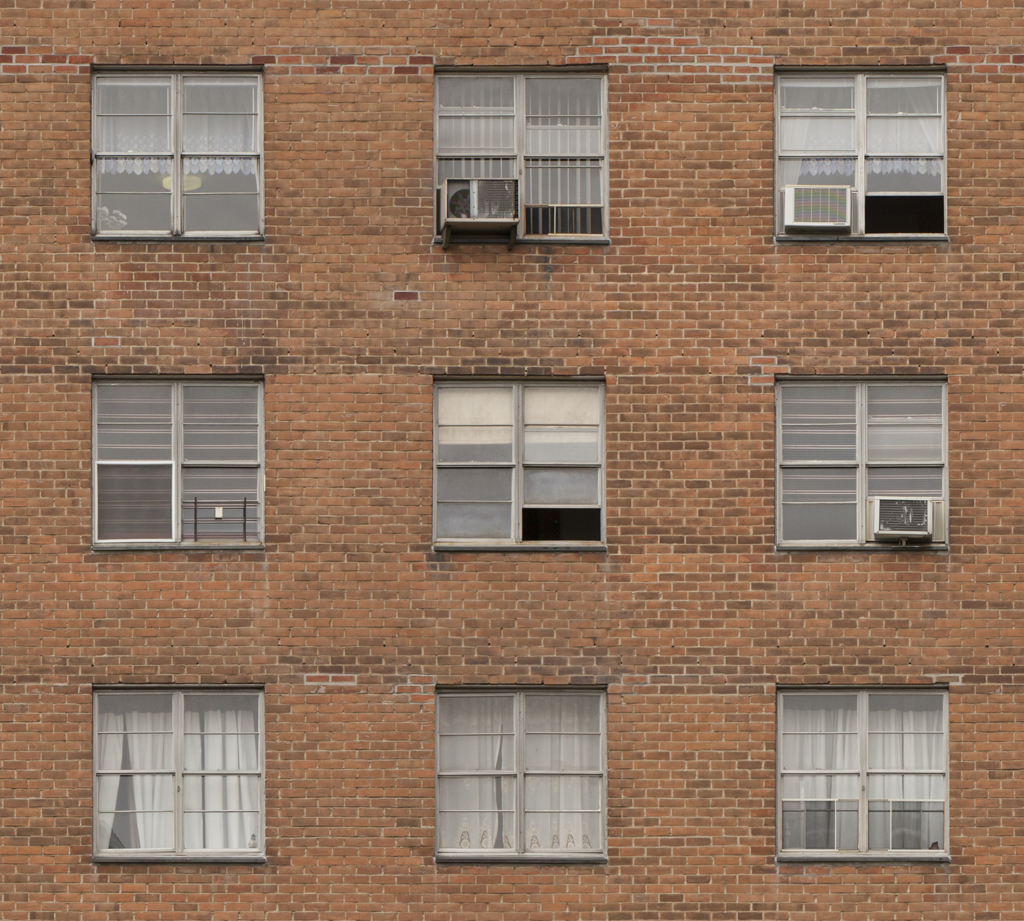
\includegraphics{pics/beamvr_damaged_texture}
    \caption{Beam VR - Damaged Texture}
    \label{fig:beamvr_damaged_texture}
\end {figure}

\begin {figure}
    \centering
    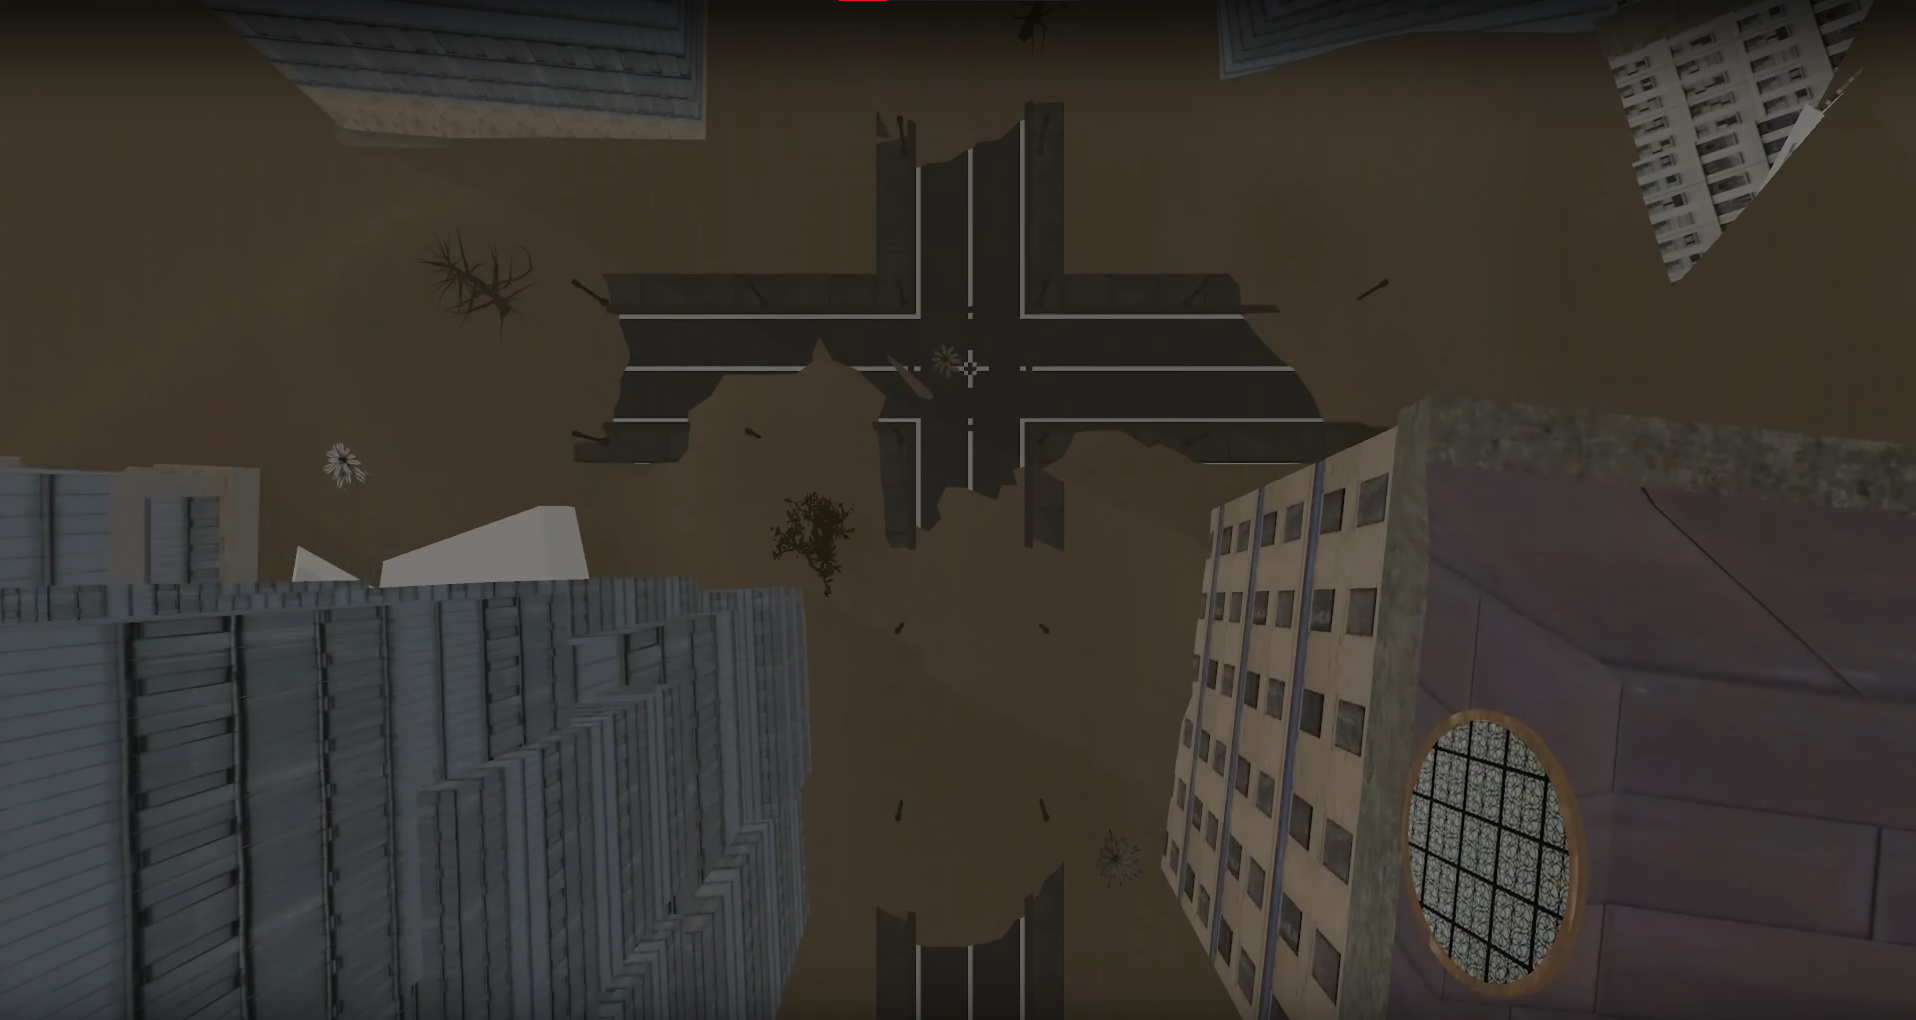
\includegraphics[scale=0.3]{pics/beamvr_apocalypse-overview}
    \caption{Beam VR - Apocalypse Map}
    \label{fig:beamvr_apocalypse_map}
\end {figure}

\section{Sound Design}\label{sec:sound}
\setauthor{Florian Beckerle}
Ohne Sound Design würden die Maps von BeamVR unrealisitsch wirken, da in einer Stadt Lärm an der Tagesordnung steht.
In der virtuellen Umgebung der verwendeten Game Engine existieren anfangs keine Geräusche, diese m\"ussen von den Entwicklern selber erstellt und eingef\"ugt werden.


Es gibt viele verschiedene Arten Sound Design zu benutzen wie zum Beispiel die Ger\"ausche, die der Anwender selbst in der virtuellen Welt verursacht.
Wenn sich der Spieler bewegt, sollten Fußstapfen zu h\"oren sein.
Diese klingen je nach Bodentyp unterschiedlich.
Besteht der Boden aus Holz, wird man ein h\"olzernes Klopfen und Knarren h\"oren.
Ist der Boden jedoch mit Gras bedeckt, wird ein Rascheln abgespielt.
Zus\"atzlich wird der gesteuerte Charakter außer Atem sein, wenn gelaufen wurde oder gerade ein Sprung ausgef\"uhrt wird.
Das wird mithilfe von Atem-Geräuschen umgesetzt.

Bei Umgebungen ist es wichtig, dass die Welt nicht leer klingt, sondern mit situationsbedingten Hintergrundger\"auschen voller Leben erscheint.
Es gibt jedoch auch Situationen, in denen gezielt wenig Umgebungsger\"ausche benutzt werden, um zum Beispiel eine W\"uste oder eine verlassene Stadt noch einsamer und trostloser darzustellen.

Um die Stimmung noch genauer steuern zu k\"onnen, kann Musik benutzt werden.
Wenn der Spieler auf einem Pferd durch eine Weide reitet, kann eine dramatische und inspirierende Musik benutzt werden, um den Moment noch besser und cinematischer wirken zu lassen.

Die Informationen für die Absätze wurden hier gefunden ~\cite{GK_Media_Factory_Sound_Design_2022}.

\subsection{Apocalypse}\label{subsec:apocalypse-background-sound}
\setauthor{Florian Beckerle}
Die Musik in der Apocalypse Map ist stark an das Horror Genre angelegt.
Die Melodie ist jedoch nicht wirklich existent, stattdessen existiert ein durchgehendes pfeifendes Ger\"ausch, welches unterbewusst das Spannungslevel erh\"oht.
Der Spieler f\"uhlt sich etwas unbehaglich und alleine.
Dadurch wirkt die Stadt, neben den br\"ockelnden H\"ausern, zus\"atzlich noch mehr verlassen.

Da die Sicht in dieser Map stark durch einen gelblichen Nebel, der wie ein Sandsturm wirkt, eingeschr\"ankt ist, kann man im Hintergrund den Wind pfeifen h\"oren.

\subsection{City}\label{subsec:day-night-background-sound}
\setauthor{Florian Beckerle}
Die Hintergrundger\"ausche der Tag und Nacht Version der Stadt sind sehr \"ahnlich.
Der Spieler kann Motorr\"ader und Autos auf den Straßen vorbeifahren h\"oren.
Hin und wieder kann man Menschen, die man nicht sehen kann, bei kurzen Gespr\"achen miteinander zuh\"oren und ein Kind husted im Hintergrund.

\subsection{Event}\label{subsec:building-collapse-sound}
\setauthor{Florian Beckerle}
Um spezifische Events, also bestimmte Dinge, welche in der Welt passieren, f\"ur den Benutzer besser erkennbar zu machen, wurden zus\"atzlich Ge\"ausche eingef\"ugt.
Auf der Apocalypse Map sind zusammenbrechende Geb\"aude zu h\"oren, um die schlechte Instandhaltung der verlassenen Stadt erneut zu verdeutlichen.
Aber wenn der Benutzer genauer hinsieht kann man, wenn diese Sounds h\"orbar sind, auch tats\"achlich eine kleine Auswahl an Bauwerken br\"ockeln sehen.

\section{Effects}\label{sec:effects}
\setauthor{Florian Beckerle}
Unity bietet verschiedene M\"oglichkeiten, um das Aussehen der Applikation zu beeinflussen.
Mithilfe von Post Processing kann man Effekte zu dem Buffer der Kamera, also dem aktuellen Frame, der gerade aufgenommen wurde, hinzuf\"ugen bevor etwas am Bildschirm angezeigt wird.
Eine kleine Auswahl dieser Effekte sind zum Beispiel Bloom, Grain oder Color Grading.
~\cite{Unity_Post_Processing_2022}

Post Processing kann global angewandt werden, somit werden die eingestellten Effekte \"uber die komplette Spielwelt angezeigt.
Um die Effekte auf einen bestimmten Bereich zu begrenzen, muss ein Collider erstellt und platziert werden.
Wenn die Kamera in diesem Collider ist, wird das angezeigte Bild mit den eingetellten Effekten versehen.
~\cite{Unity_Post_Processing_Volumes_2022}

Der Bloom Effekt wird dazu benutzt, um sehr helle Stellen und Objekte, wie bei einer echten Kamera, ausgebrannt darstellen zu können.
Hierbei wirkt das Objekt etwas verschwommen und durch die Helligkeit ist kaum etwas zu erkennen, siehe Abb. ~\ref{fig:unity-post-processing-bloom}.
\begin {figure}
    \centering
    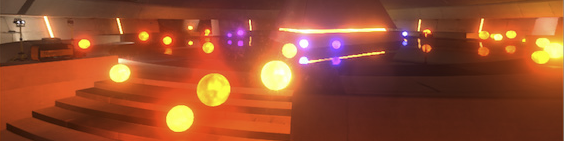
\includegraphics[scale=0.9]{pics/unity-post-processing-bloom}
    \caption{Unity - Post Processing Bloom}
    \label{fig:unity-post-processing-bloom}
\end {figure}
Dieser Effekt kann mithilfe von verschiedenen Parametern angepasst werden.
Die Intensität steuert die Stärke des Effektes, also wie stark das Bild verändert wird.
Der Treshhold filtert alle Pixel, welche unter einem bestimmten Helligkeitsniveau liegen, heraus.
Diese Pixel sind nicht von den Änderungen betroffen.
Wenn Soft Knee auf 1 gestellt wird, ist der Übergang zwischen Pixeln, die durch den Treshhold gefiltert werden, weicher.
Bei 0 befindet sich die Grenze genau auf dem eingestellten Wert.
Der Radius beeinflusst die Ausbreitung des Blooms von einem hellen Objekt aus.
Es kann zusätzlich ein Lens Dirt Effekt angewandt werden, hierbei entstehen Flecken in den hellen Bereichen, siehe Abb. ~\ref{fig:unity-post-processing-lens-dirt}.
~\cite{Unity_Post_Processing_Bloom_2022}

\begin {figure}
    \centering
    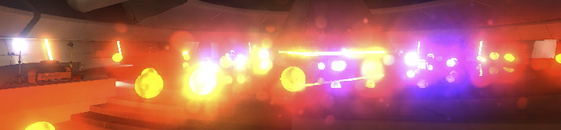
\includegraphics[scale=0.9]{pics/unity-post-processing-lens-dirt}
    \caption{Unity - Post Processing Lens Dirt}
    \label{fig:unity-post-processing-lens-dirt}
\end {figure}

Grain fügt dem angezeigten Bild einen Noise Effekt hinzu.
Hierfür wird ein nahtloses Rauschen angewandt, welches Unvollkommenheiten von Filmbändern ähnelt, siehe Abb. ~\ref{fig:unity-post-processing-grain}.
\begin {figure}
    \centering
    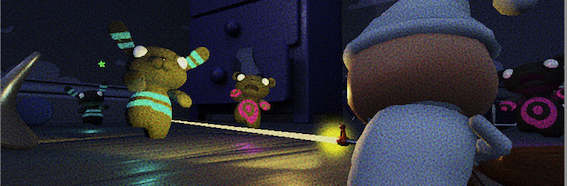
\includegraphics[scale=0.9]{pics/unity-post-processing-grain-on}
    \caption{Unity - Post Processing Grain}
    \label{fig:unity-post-processing-grain}
\end {figure}
Dieser Effekt kann ebenfalls mithilfe von verschiedenen Attributen verändert werden, siehe Abb. ~\ref{fig:unity-post-processing-grain-ui}.
Intensity steuert die Sichtbarkeit des Rauschens im Bild.
Luminance Contribution steuert das Rauschen abhängig von der Helligkeit einer Stelle im Bild.
Bei einem niedrigen Wert ist in dunklen Gebieten kaum Rauschen zu sehen.
Die Größe der Partikel wird vom Size Parameter gesteuert.
\begin {figure}
    \centering
    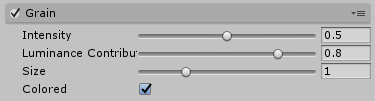
\includegraphics[scale=0.9]{pics/unity-post-processing-grain-ui}
    \caption{Unity - Post Processing Grain UI}
    \label{fig:unity-post-processing-grain-ui}
\end {figure}
~\cite{Unity_Post_Processing_Grain_2022}

Color Grading wird für die Korrektur von Farben und Helligkeit, eines Bildes verwendet.
Ein Beispiel für die Auswirkungen dieses Effekts sieht man in Abbildung ~\ref{fig:unity-post-processing-color-grading-example}.
Der linke Teil des Bildes wurde bearbeitet, der rechte Teil zeigt die ursprünglichen Farben des Bildes an.
Der linke Teil des Bildes wurde bearbeitet, der rechte Teil zeigt die ursprünglichen Farben des Bildes an.
Color Grading hat 5 verschiedene Sektionen, mit welchen genauere Einstellungen getroffen werden können.
Darunter fallen Tonemapping, Basic, Channel Mixer, Trackballs und Grading Curves.
~\cite{Unity_Post_Processing_ColorGrading_2022}
\begin {figure}
    \centering
    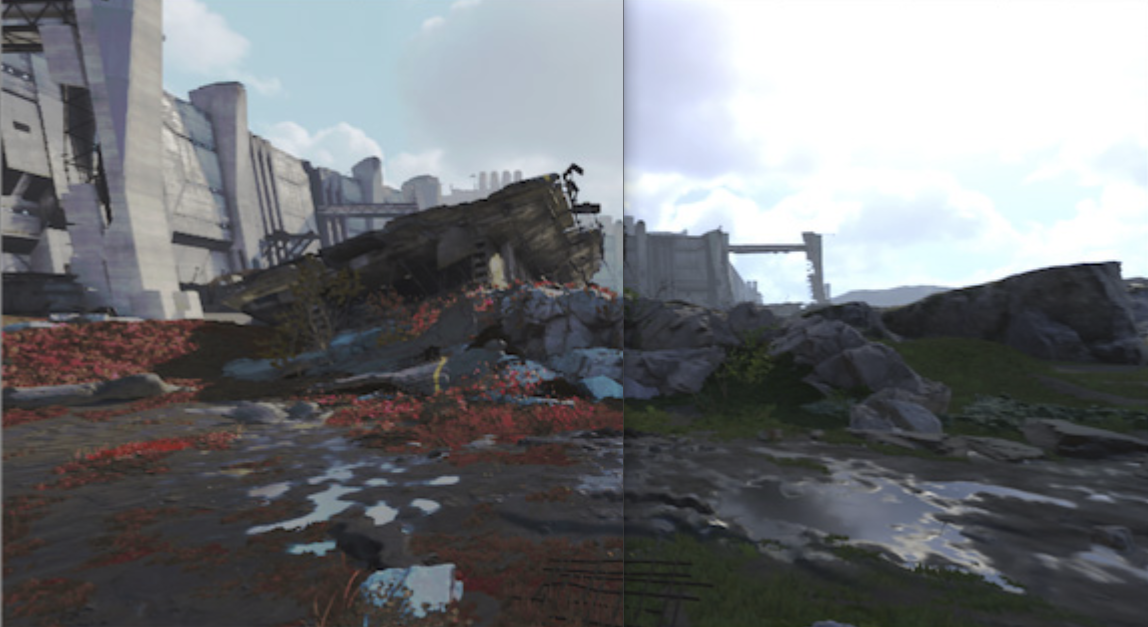
\includegraphics[scale=0.4]{pics/unity-post-processing-color-grading-before-after}
    \caption{Unity - Post Processing Color Grading Example}
    \label{fig:unity-post-processing-color-grading-example}
\end {figure}

Tonemapping beschreibt den Prozess, in welchem HDR Werte eines Bildes so umgewandelt werden, um auf einem Bildschirm dargestellt werden zu können.
Es werden dabei drei Modes zur Verfügung gestellt.
Der Neutral Tonemaper wandelt die Werte, mit möglichst geringem Einfluss auf Farbe und Sättigung, um und verwendet eine Tonemapping Curve, siehe Abb. ~\ref{fig:unity-post-processing-neutral-tonemapper-ui}.
Black In und White In steuern dabei die inneren weißen und schwarzen Kontrolpunkte, Black Out und White Out steuern die äußeren Punkte.
%Mit dem White Level kann auf einen weißen Punkt vor der Kurve eingestellt werden.
White Clip stellt auf einen weißen Punkt nach der Kurve ein.
\begin {figure}
    \centering
    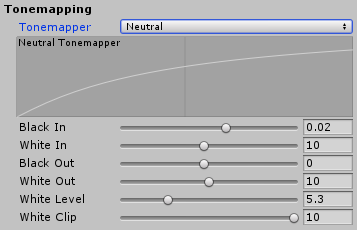
\includegraphics[scale=0.9]{pics/unity-post-processing-color-grading-neutralTonemapper}
    \caption{Unity - Post Processing Neutral Tonemapper UI}
    \label{fig:unity-post-processing-neutral-tonemapper-ui}
\end {figure}

Der Filmic (ACES) Tonemapper verwendet Schätzwerte  des ACES Tonemappers, um ein filmisches Aussehen zu erreichen.
Das Resultat ist ein höherer Kontrast und es wird Einfluss auf die Farbe und Sättigung des Bildes genommen.
Dieser Tonemapper besitzt keine Einstellungsmöglichkeiten, siehe Abb. ~\ref{fig:unity-post-processing-filmic-aces-tonemapper-ui}.

\begin {figure}
    \centering
    
\includegraphics[scale=0.9]{pics/unity-post-processing-color-grading-filmic}
    \caption{Unity - Post Processing Filmic (ACES) Tonemapper UI}
    \label{fig:unity-post-processing-filmic-aces-tonemapper-ui}
\end {figure}

Der Basic Tonemapper stellt simple Einstellungsmöglichkeiten zur Verfügung und ist ein empfohlener Startpunkt für Farbkorrekturen.
Es können Einstellungen wie Post Exposure, Temperature, Tint, Hue Shift, Staturation und Contrast eingestellt werden, siehe Abb. ~\ref{fig:unity-post-processing-basic-tonemapper-ui}.
\begin {figure}
    \centering
    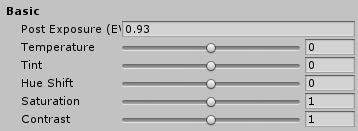
\includegraphics[scale=0.9]{pics/unity-post-processing-color-grading-basicTonemapper}
    \caption{Unity - Post Processing Basic Tonemapper UI}
    \label{fig:unity-post-processing-basic-tonemapper-ui}
\end {figure}

Post Exposure stellt die allgemeine Belichtung der Scene in EV Einheiten dar.
Dieser Effekt wird erst nach den HDR Effekten, aber vor dem Tonemapping, eingesetzt, damit die vorherigen Effekte nicht beeinflusst werden.
Die Temperatur setzt die White Balance zu einer beliebig eingestellten Farbtemperatur.
Mithilfe von Tint kann ein grüner oder magenta Tint im Bild korrigiert werden.
Hue Shift verschiebt das HUE aller Farben, während Saturation die Intensität dieser beeinflusst.
Der Contrast erweitert oder verkleinert die Breite zwischen den dargestellten Farben.

Mithilfe des Channel Mixers kann der Einfluss der einzelnen Farbkanäle, welche Rot, Grün und Blau sind, auf das gesamte Bild eingestellt werden.
Wie in Abb. ~\ref{fig:unity-post-processing-channel-mixer-ui} zu sehen ist, kann dabei jeder Farbkanal einzeln mittels eines Schiebereglers verändert werden.
Ein Beispiel für die Auswirkungen dieses Effekts ist in Abb. ~\ref{fig:unity-post-processing-channel-mixer} zu erkennen.
\begin {figure}
    \centering
    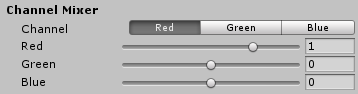
\includegraphics[scale=0.9]{pics/unity-post-processing-channel-mixer-ui}
    \caption{Unity - Post Processing Channel Mixer UI}
    \label{fig:unity-post-processing-channel-mixer-ui}
\end {figure}

\begin {figure}
    \centering
    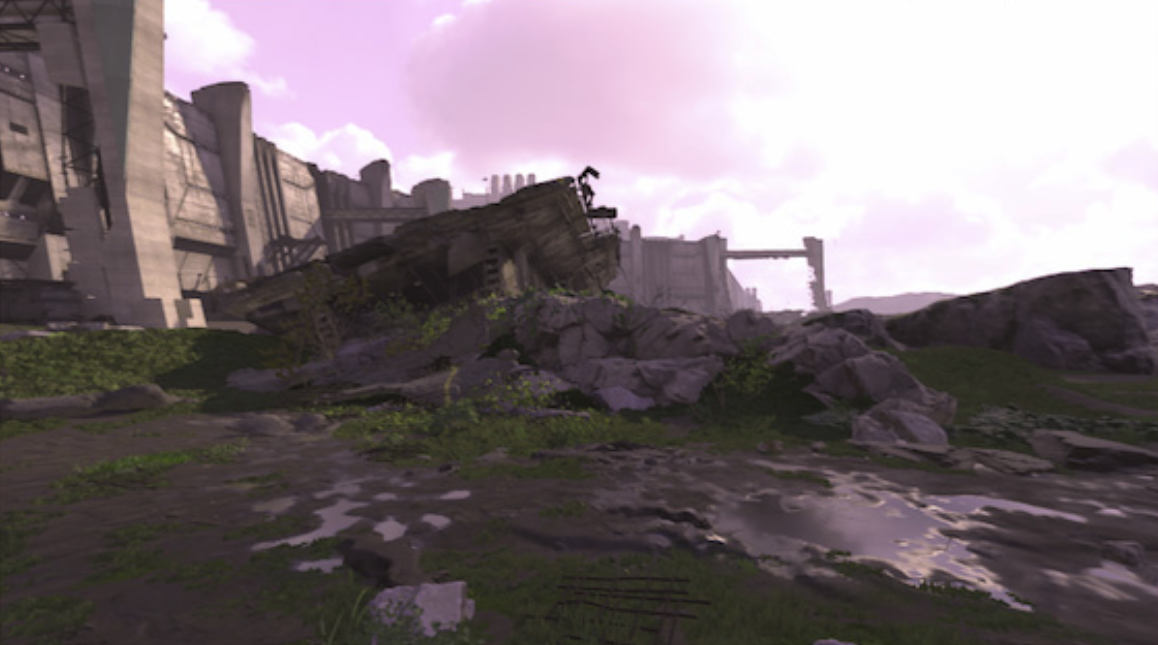
\includegraphics[scale=0.4]{pics/unity-post-processing-channel-mixer-example}
    \caption{Unity - Post Processing Channel Mixer}
    \label{fig:unity-post-processing-channel-mixer}
\end {figure}

Mithilfe von Trackballs kann man ein 3-Wege Color Grading in einem Linearen oder Logarithmischen System vornehmen.
Bei der Logarithmus Variante werden die Farbverteilung und der Contrast komprimiert um einen Color-Timing Process, welcher von optischen Film Druckern erzeugt wird, zu simulieren, siehe Abb. ~\ref{fig:unity-post-processing-trackballs-log}.
Hierbei kann mit Power das Gamma und mit Offset das Signal beeinflusst werden.
\begin {figure}
    \centering
    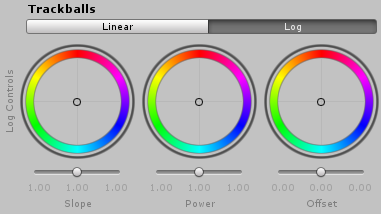
\includegraphics[scale=0.9]{pics/unity-post-processing-trackballs-log}
    \caption{Unity - Post Processing Trackballs Log}
    \label{fig:unity-post-processing-trackballs-log}
\end {figure}
Die Lineare Methode wurde für linear-encododed Data optimiert, siehe Abb. ~\ref{fig:unity-post-processing-trackballs-linear} für das UI.
Mithilfe von Lift kann das gesamte Signal verschoben werden.
Gamma beeinflusst wieder die mittleren Töne und Gain verstärkt das Signal.
\begin {figure}
    \centering
    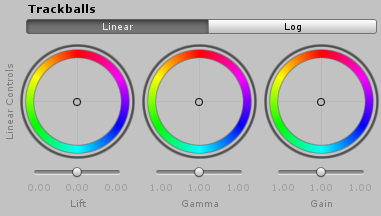
\includegraphics[scale=0.9]{pics/unity-post-processing-trackballs-linear}
    \caption{Unity - Post Processing Trackballs Linear}
    \label{fig:unity-post-processing-trackballs-linear}
\end {figure}

Mithilfe von fünf verschiedenen Grading Curves können YRGB, Hue vs Hue, Hue vs Sat, Sat vs Sat und Lum vs Sat verändert werden.
Hierbei handelt es sich jedesmal um eine Kurvendarstellung, in welcher man weitere Punkte setzen und damit den Verlauf der Kurve beeinflussen kann, siehe Abb. ~\ref{fig:unity-post-processing-grading-curve-example}.
\begin {figure}
    \centering
    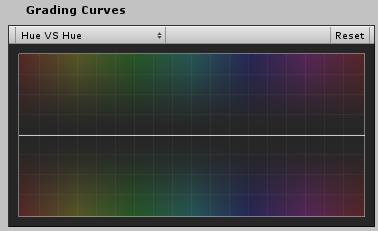
\includegraphics[scale=0.9]{pics/unity-post-processing-grading-curve-example}
    \caption{Unity - Post Processing Grading Curve Example}
    \label{fig:unity-post-processing-grading-curve-example}
\end {figure}
Bei der YRGB Kurve kann durch die Manipulation des Graphen der Contrast und die Helligkeit des Bildes eingestellt werden.
Die Hue vs Hue Kurve bietet die Möglichkeit, Farbbereiche zu verfeinern oder auszutauschen.
Um eine bestimmte Farbe besonders hervorzuheben oder einen monochromatischen Effekt zu erreichen, wird die Hue vs Sat Kurve verwendet.
Bei der Sat vs Sat Kurve werden einfache Veränderungen der Farbe wie beim Color Grading vorgenommen.
Die letzte Option heißt Lum vs Sat Kurve und ermöglicht es, in bestimmten Gebieten die Sättigung zu verringern, wie zum Beispiel in dunklen Stellen.

\subsection{Nebel}\label{subsec:fog-effect}
\setauthor{Florian Beckerle}
Unity bietet mehrere M\"oglichkeiten, Nebel darzustellen, zum Beispiel mittels Post Processing, oder mithilfe der Lighting Einstellungen.
F\"ur BeamVR wurde die zweite Variante verwendet, da der Nebel in BeamVR kein Hauptaugenmerk ist und mithilfe dieser Methode das Einstellen für BeamVR schneller ging.
~\cite{Unity_Lighting_Window_2022}

Mittels Post Processing wird ein Screen-Space Nebel Effekt in der Tiefen-Texture der Kamera erstellt, siehe Abb. ~\ref{fig:unity_post_processing_fog}.
Screen-Space bedeutet, dass die Position auf dem Bildschirm und nicht in der dreidimensionalen Welt berechnet wird.
~\cite{Unity_Fog_2022}

\begin {figure}
    \centering
    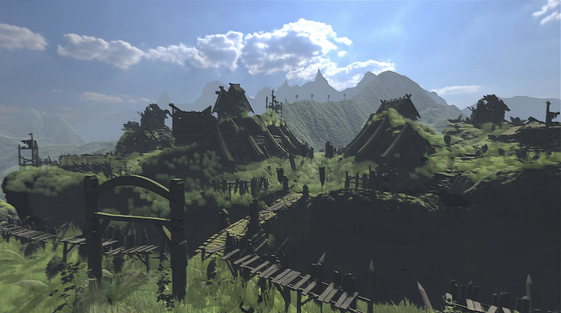
\includegraphics[scale=0.9]{pics/unity-post-processing-fog}
    \caption{Unity - Post Processing Fog}
    \label{fig:unity_post_processing_fog}
\end {figure}
Unter dem Begriff Map versteht man eine Umgebung in einer Spielwelt, in diesem Fall wird auf die Szenen, in welchen die Städte platziert sind, verwiesen.
Auf fast jeder Map von BeamVR wurde dieser Nebel verwendet.
In der Nacht Map wird mithilfe dieses Effekts ein leichter Nebel dargestellt, was zur abendlichen Stimmung beitr\"agt.
Bei Apocalypse ist der Nebel viel dichter und stellt einen Sandsturm dar. Zus\"atzlich wurde dieser gelb gef\"arbt, um noch mehr an Sand zu erinnern, siehe Abb. ~\ref{fig:beamvr_yellow_fog}.

\begin {figure}
    \centering
    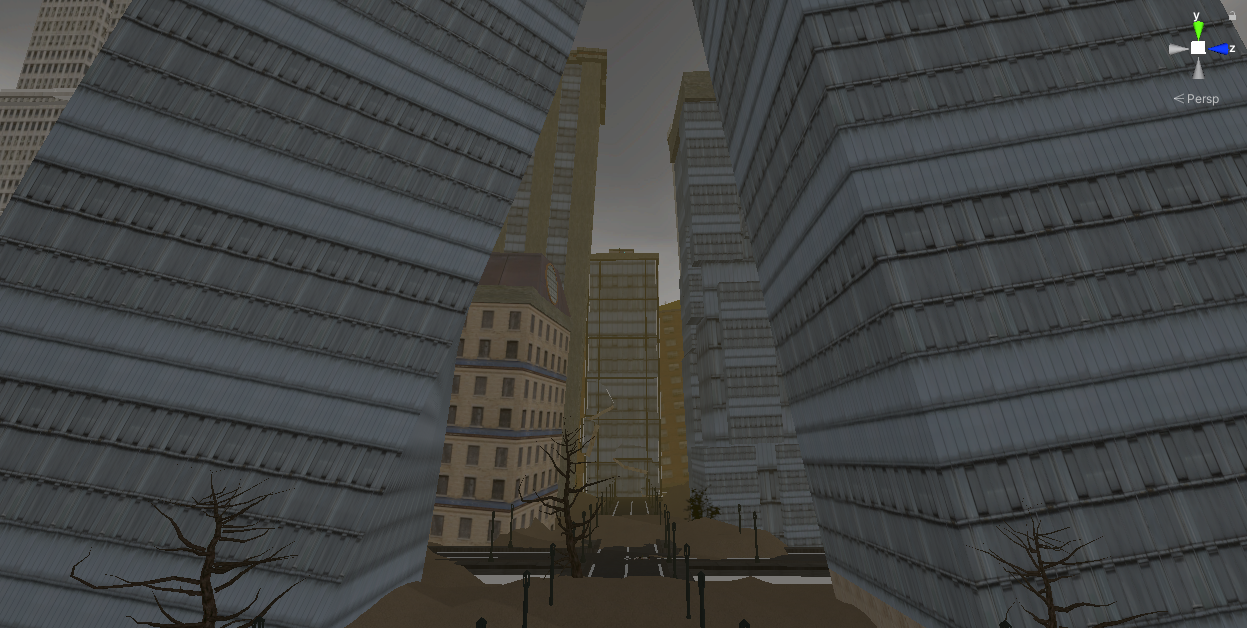
\includegraphics[scale=0.3]{pics/beamvr_yellow_fog}
    \caption{Beam VR - Yellow Fog}
    \label{fig:beamvr_yellow_fog}
\end {figure}

Mittels der High Definition Render Pipeline, welche auch als HDRP bezeichnet wird, kann ebenfalls Nebel eingestellt werden.
Hierfür wird die Volume Framework benötigt, in welcher ein Nebel Overrride hinzugefügt wird.

Diese Framework bietet einige verschiedene Optionen zur Beeinflussung des Nebels, siehe Abb. ~\ref{fig:unity-hdrp-fog}.
Die Option Enable wird verwendet, um den Effekt zu aktivieren oder deaktivieren.
Die Fog Attenuation Distance bestimmt die Dichte und die Sichtweite im Nebel.
Ab der eingestellten Distanz hat der Nebel bereits 63\% des Umgebungslichts absorbiert.
Dichte und Sichtweite bleiben bis zu einer definierten Base Height constant, erst ab dieser ist eine exponentielle Abnahme beider Attribute erkennbar.
Die Maximum Height und Max Fog Distance bestimmen die Stärke des Abfalls und die Distanz des Nebels.
Mittels des Color Modes kann die Farbe des Nebels beeinflusst werden.
Bei Sky Color wird die Farbe automatisch an den Himmel angepasst, während bei constant Color eine eigene Farbe eingestellt werden kann.

Volumetric Fog kann mittels der gleichnamigen Option aktiviert werden.
Die Albedo Option setzt dabei die Farbe des Nebels, mit welcher das Licht gestreut wird.
Lichter werden, mit zunehmender Dichte des Nebels, schneller abgedunkelt.
Anisotropy steuert die Streuung des Lichtes.
0 streut das Licht gar nicht, 1 streut das Licht vorwärts und -1 streut rückwärts.
Mittels eines Filters kann eine Unschärfe der eingehenden Lichter geschaffen werden, damit ein weicherer Übergang zustande kommt.
~\cite{Unity_HDRP_Fog_2022}

\begin {figure}
    \centering
    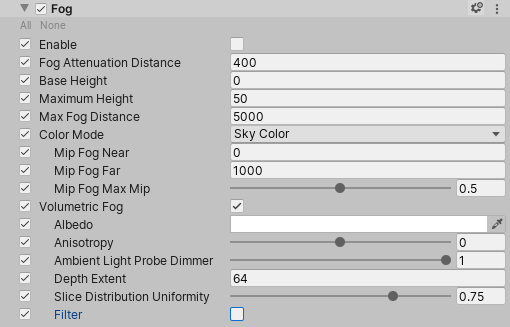
\includegraphics[scale=0.9]{pics/unity-hdrp-fog}
    \caption{Unity - HDRP Fog}
    \label{fig:unity-hdrp-fog}
\end {figure}


\subsection{Lichter}\label{subsec:light-effect}
\setauthor{Florian Beckerle}
In der Nacht Map wurden die von Unity bereitgestellten Point-Lights als Straßenlichter benutzt.
Point Lights k\"onnen mithilfe eines Radius auf einen bestimmten kreisf\"ormigen Bereich eingegrenzt werden.
Weiters wird mithilfe der Lichtst\"arke die Wirkkraft des Lichtes in diesem Gebiet genauer bestimmt.
Dank dieser Eigenschaften war das Point Light f\"ur die Aufhellung der Straßen, siehe Abb. ~\ref{fig:beamvr_street_lights}.
~\cite{Unity_PointLights_2022}
\begin {figure}
    \centering
    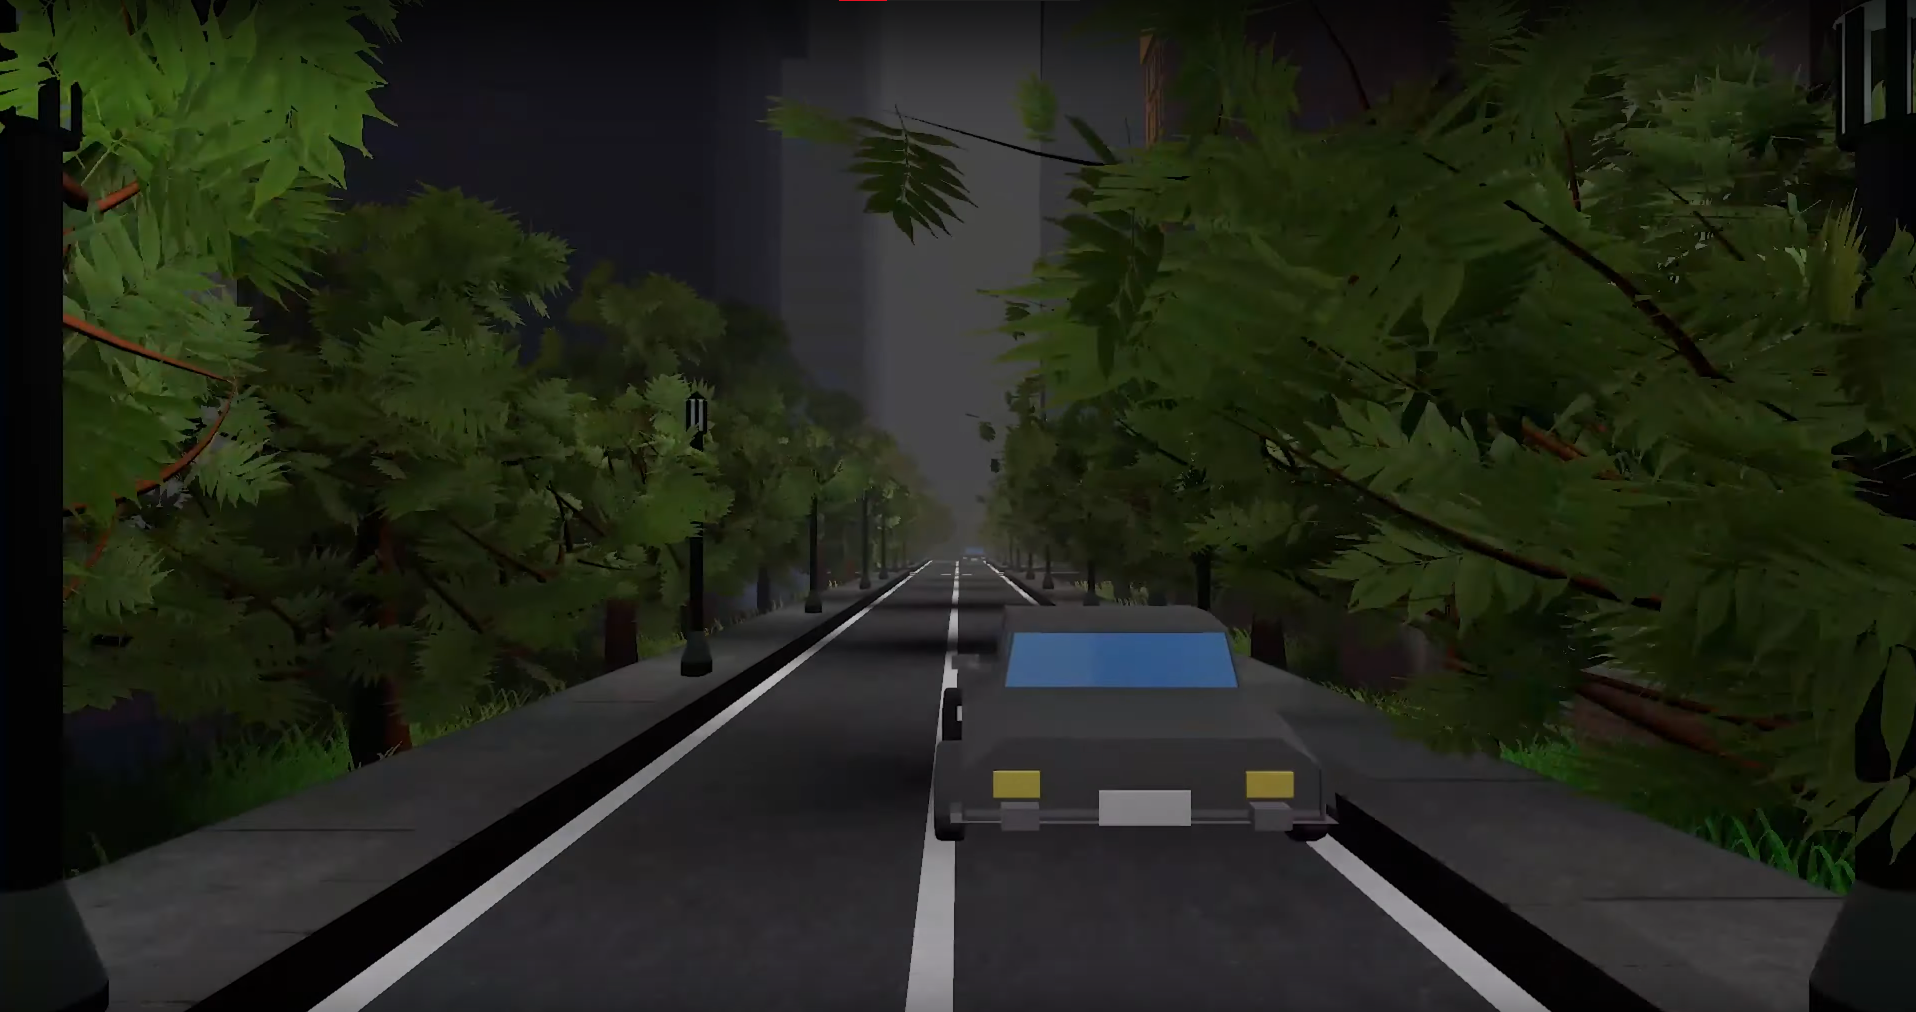
\includegraphics[scale=0.3]{pics/beamvr_point_lights}
    \caption{Beam VR - Street Lights}
    \label{fig:beamvr_street_lights}
\end {figure}

\subsection{Wind}\label{subsec:wind-effect}
Damit sich die B\"aume und B\"usche in BeamVR wie im Wind bewegen, werden Unitys Wind Zones ben\"otigt.
Diese Zonen sind bestimmte Bereiche, in welchen eine Windrichtung, Windst\"arke und Turbulenz definiert wird.
Die eingestellten Effekte werden dann auf alle Objekte angewandt, die mithilfe des Terrains oder Particle Systems iniziiert wurden.
~\cite{Unity_WindZones_2022}

\section{Unity Prefabs}
\label{sec:prefabs}
\setauthor{Quirin Ecker}

In Unity gibt es ein System welches dem Entwickler oder der Entwicklerin erlaubt eine bestimmte Zusammenstellung von 3d Elementen zu speichern und mehrmals in verschiedenen Szenen zu verwenden.
Diese Zusammenstellungen von 3d Elementen heißen auch Prefabs.
Wird dieses Prefab verändert, wird es an jeder platzierten Stelle aktualisiert.
Es werden dabei die Komponenten und Positionen der einzelnen Elemente relativ zu dem Prefab gespeichert.

Prefabs können auch überschrieben werden an der Stelle wo sie platziert worden sind.
Aus Erfahrung zeigt sich aber, dass dies mit Vorsicht zu genießen ist, da lokale Änderungen nicht mehr global überschrieben werden.
Somit haben globale Änderungen keinen wirklichen Einfluss auf das lokale Prefab.
Außerdem können Prefabs auch ineinander verschachtelt werden~\cite{Unity_Prefabs}.

In der BeamVR Applikation wird dieses System an mehreren Stellen verwendet.
Diese Prefabs wurden beispielsweise in der BeamVR Applikation für einzelne Elemente, welche in allen Karten existieren, benutzt.
Alle diese Elemente werden in ein sogenanntes Game Prefab gruppiert, welches in allen Karten platziert wird.

Folgend werden das Game Prefab und zwei weitere für BeamVR relevante Prefabs noch genauer beschrieben.

\subsection{Game}\label{subsec:game-prefab}

Wie bereits beschrieben befinden sich alle Game relevant Elemente in dem Game Prefab.
Somit wird dieses Prefab in allen Karten Szenen verwendet.
Nur in der Menü- und Setup-Szenen wird dieses Prefab nicht gebraucht.

Folgend sind die wichtigsten Elemente des Game Prefab aufgelistet:

\begin{itemize}
    \item \textbf{Beam:} Der Beam ist der virtuelle Balken, der von dem Hochhaus absteht.
    \item \textbf{Collider:} Die Collider sind Elemente, welche Aktionen auslösen, wenn ein anderes Element mit diesen kollidiert.
    Visuelle sind diese Collider unsichtbar.
    \item \textbf{GameCameraRig:} Das~\emph{GameCameraRig} ist ein weiteres Prefab, welches für VR spezifische Elemente zuständig ist.
\end{itemize}


\subsection{GameCameraRig}\label{subsec:game-camera-rig}

Wie bereits im Game Prefab beschrieben ist das GameCameraRig Prefab ein bestandteil des Game Prefab und beinhaltet alle VR spezifischen Elemente.
Dieses Prefab ist ein abgeändertes CameraRig Prefab, welches bereits von dem SteamVR Plugin zur Verfügung gestellt worden ist.
Das Prefab an sich soll den VR Raum darstellen.

Folgende sind die wichtigsten Elemente des GameCameraRig Prefab aufgelistet:

\begin{itemize}
    \item \textbf{Controller:} Die Controller sind Elemente welche eine SteamVR Controller Script-Component beinhalten.
    Durch dieses Script befindet sich dieses Element in der richtigen Position und Orientierung relativ zu der VR Fläche.
    \item \textbf{Camera:} Genauso wie die Controller Elemente besitzt das Camera Element auch ein Script.
    Mit diesem Script nimmt die Kamera die Position und Orientierung des Headsets relativ zur VR Fläche an.
    Diese Kamera ist auch für die Sicht des Spielers zuständig.
    \item \textbf{Tracker Objekte} Diese Elemente haben ebenfalls wieder ein ähnliches Script.
    Durch dieses Script befindet sich dieses Element in der gleichen Position und Orientierung des physischen Tracker.
    In der Script Komponente kann in einem Auswahlmenü der richtige Tracker eingestellt werden.
    \item \textbf{Spieler Modell:} Das Spieler Modell ist das Modell, welches nach dem Kalibrieren des Full-Body-Trackings die Pose des Spielers einnimmt.
    \item \textbf{VRIK Calibration Controller:} Bei diesem Element befindet sich ein Script-Component, in dem das Full-Body-Tracking konfiguriert werden kann.
    Für mehr Informationen wird auf Abschnitt~\ref{sec:final-ik-plugin} verwiesen.
\end{itemize}

\subsection{MenuCameraRig}\label{subsec:menu-camera-rig}

Das MenuCameraRig ist genauso wie das GameCameraRig eine Abänderung des von SteamVR Plugin bereitgestellte CameraRig.
Im Gegensatz zum GameCameraRig wird das MenuCameraRig nicht in den 3 Karten verwendet.
Das MenuCameraRig wird in den Menü-Szenen verwendet und besteht aus Menü und VR spezifische Elemente.

Viele Elemente sind gleich wie bei dem GameCameraRig.
Der große Unterschied des MenuCameraRig ist, dass die Controller noch weitere Script-Componenten beinhalten.
Diese sind Input Scripts welche für den Auswahlstrahl und das Auswählen der Menü-Elemente verantwortlich sind.

%TODO: (Quirin Ecker)(optional) Möglichkeit für ein Bild eines Inputstrahls

Weiters sind viele der game-spezifischen Elemente in diesem Prefab nicht vorhanden.
Beispielsweise gibt es keine Full-Body-Tracking Elemente, wie das Spieler-Modell und der VRIK-Calibration-Controller.
